% Единый отчет по реализованным пунктам курса «Информационный поиск».
% Сборка из reports/pdf: два запуска pdflatex search_system.tex.
% Оригинальный стиль: https://github.com/toshunster/MAI-IR/tree/main/report_pattern
\documentclass[pdf,unicode,12pt,a4paper,oneside,fleqn]{article}
\usepackage{../source/styles/report-pattern}
\usepackage{tabularx,booktabs,needspace}
\hypersetup{unicode=true,
  pdftitle={Поисковая система для технического корпуса},pdfauthor={Д. А. Кулешов}}
\emergencystretch=2em
\newcolumntype{Y}{>{\raggedright\arraybackslash}X}
% Короткие примеры и команды не разрываются между страницами.
\BeforeBeginEnvironment{lstlisting}{\par\noindent\begin{minipage}{\linewidth}}
\AfterEndEnvironment{lstlisting}{\end{minipage}\par}
\newcommand{\labsection}[2]{\par\Needspace{9\baselineskip}\setcounter{section}{\numexpr#1-1\relax}\section{#2}}
\newcommand{\partlabel}[1]{\par\Needspace{4\baselineskip}\medskip\textbf{#1.}\quad}
\urlstyle{tt}
\DeclareRobustCommand{\code}[1]{\expandafter\nolinkurl\expandafter{\detokenize{#1}}}
\newcommand{\GiB}{\,\text{ГиБ}}
\newcommand{\KiB}{\,\text{КиБ}}
\begin{document}
\hypersetup{pageanchor=false}

\begin{titlepage}
\begin{center}
\bfseries

{\Large Московский авиационный институт\\ (национальный исследовательский университет)

}

\vspace{48pt}

{\large Факультет информационных технологий и прикладной математики
}

\vspace{36pt}

{\large Кафедра вычислительной математики и~программирования

}


\vspace{48pt}

Отчет по лабораторным работам по курсу \enquote{Информационный поиск}

\vspace{18pt}

\enquote{Поисковая система для технического корпуса документов}

\end{center}

\vspace{72pt}

\begin{flushright}
\begin{tabular}{rl}
Студент: & Д.\,А. Кулешов \\
Преподаватель: & А.\,А. Кухтичев \\
Группа: & М8О-408Б-23 \\
Дата: & \\
Оценка: & \\
Подпись: & \\
\end{tabular}
\end{flushright}

\vfill

\begin{center}
\bfseries
Москва, 2026
\end{center}
\end{titlepage}

\pagebreak

\hypersetup{pageanchor=true}

\tableofcontents
\clearpage
\section*{Общая постановка и состав системы}
\addcontentsline{toc}{section}{Общая постановка и состав системы}

Цель работы состоит в создании поисковой системы для разнородных англоязычных
технических текстов. В качестве источников выбраны Wikipedia, arXiv HTML и
Microsoft Learn. Они представляют три разных жанра: энциклопедическую статью,
научную публикацию и прикладную документацию. Такое сочетание позволяет
проверить поиск на естественном языке, научной терминологии, именах программных
интерфейсов и примерах кода.

Разделы отчета соответствуют отдельным пунктам со значками-кружками в README
курса, а не номерам каталогов занятий. Сохранены исходные номера пунктов:
1--8, 10--13 и 17. Для каждого из них приведены постановка задачи, метод,
существенные этапы выполнения, проверки и выводы. Общие команды вынесены
в конец отчета, чтобы не повторять подготовку окружения в каждом разделе.

Основные компоненты обработки текста, построения индексов и поиска написаны
на C++. Python используется для поискового робота, начального анализа источников
и экспериментальной оценки качества. Для ключевых поисковых структур применены
собственные таблицы, операции над списками и структуры накопления результатов.
Строки и динамические массивы используются как контейнеры данных; готовые
поисковые движки и библиотечные хеш-таблицы ключевых структур не используются.
Единая кодировка данных и запросов - UTF-8.

Последовательность обработки имеет следующий вид:
\begin{center}
источники $\longrightarrow$ сырые HTML в MongoDB\\[3pt]
$\longrightarrow$ выделение текста, токенизация, лемматизация\\[3pt]
$\longrightarrow$ прямой индекс частот и обработанные тексты\\[3pt]
$\longrightarrow$ обратный и координатный индексы на диске\\[3pt]
$\longrightarrow$ булев, ранжированный и цитатный поиск.
\end{center}

В рассматриваемом снимке обработано 1\,132\,727 исходных документов. После
выделения текста и фильтра по минимальной длине принято 993\,923 документа,
отклонено 138\,804. Поэтому объем скачанного корпуса превышает миллион,
но поисковый индекс данного снимка содержит меньше миллиона документов.
Это различие учитывается во всех дальнейших измерениях. Порог принятия равен
100 токенам, версия правил обработки - 9.

Контрольные проверки и сравнительные замеры выполнены в Linux x86-64
под WSL2, на AMD Ryzen 5 5600 с 12 логическими процессорами; среде WSL
доступно около 15 ГиБ оперативной памяти. Сборка C++ выполняется в режиме
Release. Объем сырых HTML значительно превышает доступную память,
поэтому построение индексов организовано на внешней памяти.

\labsection{1}{Добыча корпуса документов}

\partlabel{Задание и выбор источников}
Необходимо выбрать тематически связанный корпус из нескольких источников,
получить примеры, исследовать разметку и метаданные, выделить основной текст
и оценить пригодность данных для последующего поиска. Для предварительного
анализа я использовал по 30 документов каждого источника. Анализ выполнен
в трех отдельных ноутбуках; всего исследовано 90 примеров.

Wikipedia дает обзорные определения и связи между понятиями. arXiv содержит
подробные научные статьи по компьютерным наукам и смежным дисциплинам.
Microsoft Learn дополняет корпус инструкциями, описаниями API и конфигураций.
Техническая тематика достаточно широка, поэтому корпус не сводится к одному
продукту или одному типу статьи. Вместе с тем принадлежность страницы к
источнику сама по себе не гарантирует ее тематическую чистоту.

\partlabel{Метод получения и анализа}
В предварительном исследовании Wikipedia запрашивается через MediaWiki API:
сначала выбираются страницы категорий, затем загружаются заголовок, URL,
идентификатор и текстовый \code{extract}. Сырое представление этого
\emph{ноутбука} - JSON с уже очищенным текстом. При последующем массовом
обходе робот сохраняет HTML страниц. Поэтому размеры JSON начальной выборки
нельзя напрямую сравнивать с размерами HTML массового корпуса.

Для arXiv Atom API используется как каталог публикаций и метаданных, а полный
документ загружается с адреса вида \code{https://arxiv.org/html/<id>}. Для
Microsoft Learn адреса берутся из sitemap, после чего скачиваются HTML-страницы.
При разборе я отдельно сохраняю идентификаторы и URL и отдельно получаю
содержательный текст. Навигация, стили, скрипты и повторяющиеся служебные
блоки не должны становиться поисковым содержимым.

\begin{table}[htbp]\centering
\caption{Результаты предварительной выборки; размеры в байтах UTF-8}
\begin{tabularx}{\textwidth}{Yrrr}
\toprule
Источник & Документов & Сырое представление & Выделенный текст\\
\midrule
Wikipedia, JSON & 30 & 643\,895 & 623\,248\\
arXiv, HTML & 30 & 16\,108\,664 & 2\,242\,943\\
Microsoft Learn, HTML & 30 & 1\,770\,272 & 307\,385\\
\bottomrule
\end{tabularx}
\end{table}

Среднее число слов в этих выборках составило соответственно 3\,121,37,
11\,931,97 и 1\,474,33. Здесь слова подсчитаны разделением текста по пробелам;
это исследовательская оценка, отличная от последующей технической токенизации.
Средний сырой размер равен суммарному размеру, деленному на 30: 21\,463,17,
536\,955,47 и 59\,009,07 байта соответственно. Средний объем текста равен
20\,774,93, 74\,764,77 и 10\,246,17 байта.

Для массового корпуса дополнительно подсчитана сумма поля \code{raw_size}
в MongoDB. Она равна 200\,806\,457\,750 байтам ($187{,}02\GiB$).
Это логический объем сохраненных HTML, а не размер файлов MongoDB на диске:
служебные данные и внутреннее сжатие базы в эту сумму не входят.

\begin{table}[htbp]\centering
\caption{Массовый корпус: скачанные и принятые документы}
\begin{tabularx}{\textwidth}{Yrrr}
\toprule
Источник & Скачано & Принято & HTML, ГиБ\\
\midrule
Wikipedia & 379\,764 & 373\,477 & 121,83\\
arXiv & 74\,850 & 74\,755 & 30,87\\
Microsoft Learn & 678\,113 & 545\,691 & 34,32\\
\midrule
Всего & 1\,132\,727 & 993\,923 & 187,02\\
\bottomrule
\end{tabularx}
\end{table}

\partlabel{Разбор документов и проверки}
На странице \href{https://en.wikipedia.org/wiki/Computer_science}{Computer science}
я проверил сохранение заголовка, URL и связного основного текста.
В выборке ее JSON занимает 30\,814 байт, текст - 30\,137 байт, 4\,306 слов.
Для \href{https://arxiv.org/html/2610.28435v1}{Multimodal Reranking Is a System One Decision}
основной узел находится в \code{article.ltx_document}; HTML занимает
393\,967 байт, текст - 36\,089 байт, 5\,806 слов. В статье Microsoft Learn
\href{https://learn.microsoft.com/en-us/cosmos-db/index-vector-data}{Index vector data in Cosmos DB}
содержательное наполнение выделяется из центральной области страницы;
получено 14\,273 байта текста из 61\,456 байт HTML, 2\,149 слов.

Для всех 90 примеров проверялись непустой текст, наличие идентификатора и URL,
сохранение заголовков и отсутствие основной навигации. При просмотре формул
arXiv обнаруживается потеря двумерной структуры при переводе в обычный текст.
Код и таблицы Microsoft Learn, напротив, следует сохранять: они содержат
полезные команды и имена параметров.

\partlabel{Вывод}
Источники подходят для совместного технического корпуса, но требуют разных
правил извлечения текста. Начальные 90 примеров служат проверкой метода,
а не доказательством качества всего корпуса. Существующие поиски Wikipedia
и Microsoft Learn используются далее как альтернативы в эксперименте:
это позволяет сопоставить выдачи, а не ограничиваться оценкой внешнего вида
отдельных страниц.

\labsection{2}{Поисковый робот}

\partlabel{Задание и метод}
Робот должен обнаруживать документы трех источников, сохранять оригиналы,
избегать повторов, поддерживать продолжение обхода и повторную проверку страниц.
Реализация находится в \code{src/crawler}; параметры вынесены в
\code{configs/crawler.yaml}. Используется асинхронный запуск независимых
источников, а не неограниченная параллельная отправка запросов одному серверу.

Для Wikipedia обход начинается с тематических категорий MediaWiki. В очередь
попадают страницы и разрешенные подкатегории в пределах заданной глубины.
Направление обхода ограничивается фильтрами названий категорий. Для arXiv
публикации обнаруживаются по категориям и месячным интервалам, а затем
скачивается доступная HTML-версия. Разбиение на интервалы уменьшает объем
отдельной API-выборки и позволяет сохранять точку продолжения. У Microsoft
Learn источником URL служат sitemap и даты изменения страниц.

\partlabel{Организация MongoDB}
Коллекция \code{documents} содержит сырые документы. Для каждой страницы
сохраняются источник \code{source}, идентификатор \code{source_id}, URL,
заголовок, \code{raw_html}, размер \code{raw_size}, хеш
\code{content_hash}, даты первого получения, получения текущей версии и
последней проверки. Поля \code{etag} и \code{last_modified} нужны для
условных HTTP-запросов, а \code{metadata} - для сведений конкретного источника.
MongoDB хранит документ в BSON, то есть в типизированном бинарном представлении
полей; HTML остается строкой и не превращается в извлеченный текст.

Хеш вычисляется как SHA-256 от UTF-8-байтов сохраненного HTML. Он отвечает
на вопрос об изменении содержимого, но не заменяет идентификатор страницы.
Уникальные индексы по парам \code{(source, source_id)} и \code{(source, url)}
не дают сохранить один объект повторно под тем же ключом. При этом одинаковый
текст на двух разных URL не считается автоматически одним документом.

Очередь Wikipedia хранится в \code{crawl_queue}, контрольные точки источников
и время допустимого продолжения - в \code{crawl_state}. Состояние сохраняется
в MongoDB, поэтому перезапуск не требует заново проходить весь каталог.
Смена версии стартовых правил позволяет расширить обход, не удаляя уже
скачанные документы.

\partlabel{Обновление, ограничения и возникшие проблемы}
В конфигурации задан интервал повторной проверки 7\,776\,000 секунд,
то есть 90 суток. Свежие документы пропускаются. При наличии ETag или даты
изменения робот отправляет условный запрос; ответ 304 подтверждает актуальность
без повторной загрузки тела. При ответе 200 сравнивается хеш, и измененная
страница обновляется по прежнему ключу. Робот выполняет конечный запуск;
периодичность новых запусков задается снаружи.

При работе возникали ошибки 500 API arXiv, ответы ограничения частоты и
исчерпание полезной части категорий Wikipedia. Для временных ошибок применены
повторы с увеличенной паузой, учет \code{Retry-After} и сохранение длительной
паузы источника. Обход Wikipedia расширялся тематическими категориями;
простое увеличение глубины без фильтра приводило к уходу в нетехнические темы.
Коллизии URL при разных идентификаторах обрабатываются без удаления старых
записей. Уменьшение задержек не гарантирует отсутствия блокировок: робот
соблюдает паузы и правила robots.txt, но окончательное решение остается у сайта.

\partlabel{Результат и проверка}
В снимке лингвистической обработки имеется 1\,132\,727 исходных документов.
Логирование поддерживает подробный режим и сводку за минуту. Проверки робота
покрывают конфигурацию, очереди, контрольные точки, ограничения и повторы,
обновление и обработку конфликтов. Выполнено 64 Python-теста, все прошли.
Тесты используют управляемые ответы и подмены зависимостей, а не создают
нагрузку на внешние сайты.

\partlabel{Вывод}
Робот обеспечивает возобновляемую загрузку и обновление документов без
полного повторного обхода. Тематичность Wikipedia остается приближенной,
поскольку категории образуют неоднородный граф. Сохранение оригинального HTML
позволяет улучшать обработку текста без повторной выкачки всего корпуса.

\labsection{3}{Токенизация}

\partlabel{Задание и место в обработке}
Токенизатор преобразует извлеченный текст в последовательность поисковых единиц.
Для технического корпуса недостаточно разделения по знакам пунктуации:
из \code{C++}, \code{C#}, \code{.NET} и \code{node.js} должны получаться
самостоятельные осмысленные термы. Реализация находится в языковой части
\code{src/linguistics}; одни правила используются для документов и запросов.

Перед токенизацией C++-обработчик с помощью libxml2 выбирает содержательную
область HTML по правилам источника и удаляет служебные узлы. Для Wikipedia
важен контейнер статьи, для arXiv - научный документ LaTeXML, для Microsoft
Learn - центральное содержимое. Удаление разметки и токенизация являются
разными этапами: токенизатор получает текст, а не должен распознавать HTML.

\partlabel{Алгоритм и особенности}
Текст последовательно читается как UTF-8. Декодер проверяет допустимость
многобайтных последовательностей и границы Unicode. Типографические пробелы,
кавычки и варианты дефисов приводятся к согласованному виду; поддерживается
нормализация полноширинных ASCII-символов. Слова приводятся к нижнему регистру.
Некорректные последовательности не должны приводить к чтению за границей
строки или склеиванию несвязанных фрагментов.

После определения границ слова проверяются технические конструкции.
Символы \code{::}, \code{--}, \code{/}, \code{@} и точка допускаются внутри
соответствующих конструкций по контекстным правилам. Это позволяет сохранять
имена пространств имен, параметры команд, пути, адреса и URL. Завершающая
пунктуация предложения отделяется от терма. Повторное вхождение не удаляется:
частота и порядок нужны для TF-IDF и координатного индекса.

\begin{lstlisting}
Input:  C++ and C++ use node.js with .NET.
Tokens: [c++, and, c++, use, node.js, with, .net]
\end{lstlisting}

Максимальная длина токена в текущей конфигурации равна 100 Unicode-символам.
Это ограничивает патологические идентификаторы, но не является доказательством
того, что любой короткий токен полезен. Стоп-слова сохраняются: их удаление
усложнило бы поиск фраз и изменило бы частотное распределение корпуса.

\partlabel{Измерения и тестирование}
На принятой части корпуса получено 2\,205\,065\,484 вхождения токенов,
19\,058\,577 различных токенов. Средняя длина токена составляет 5,756 символа.
Объем выделенного текста равен 15\,761\,592\,042 байтам
($14{,}68\GiB$); средний размер принятого текста - 15\,857,96 байта.

Суммарное измеренное время непосредственно токенизации составляет 231,56 с,
скорость - 66\,472,88 КиБ/с. Время измеряется через \code{std::chrono} вокруг
выделенного участка обработки. Оно не включает полное чтение MongoDB,
HTML-разбор, лемматизацию и запись результатов. Полное время сохраненного
запуска пайплайна - 27\,538,89 с, или около 7,65 ч. Сравнивать эти числа
как два времени одной и той же операции нельзя.

План тестирования включает пустые строки, различные пробелы и пунктуацию,
регистр, Unicode, поврежденный UTF-8, границы длины, технические имена,
повторения нескольких одинаковых специальных термов и соседство разных
конструкций в одном тексте. Проверяется вся последовательность токенов,
а не только наличие одного удачного совпадения.

\partlabel{Вывод}
Правила сохраняют значимые обозначения технического корпуса и одинаково
применяются к запросу и документу. В частотах всего корпуса, однако,
наблюдаются артефакты вроде \code{kmmpcjpl}. Это указывает на остаточный шум
извлечения и шаблонов отдельных страниц; высокая скорость токенизации не
означает отсутствия такого шума. Его устранение требует проверки источника
артефакта, а не произвольного удаления всех редких или необычных слов.

\labsection{4}{Лемматизация}

\partlabel{Задание и выбранный подход}
Лемматизация сводит разные словоформы к общей словарной форме, чтобы запрос
и документ совпадали независимо от числа или некоторых грамматических форм.
Например, \code{queries} должно сопоставляться с \code{query}. В отличие
от механического удаления окончания, лемматизация проверяет словарную основу
и исключения. В работе реализована словарная нормализация английского языка
без контекстного определения части речи.

\partlabel{Алгоритм и данные}
Токены поступают после токенизатора. Сначала учитываются явные технические
переопределения из \code{resources/technical_lemma_overrides.tsv}.
Затем учитываются встроенные неправильные формы, исключения WordNet
и словарь допустимых лемм:
\code{resources/wordnet_exceptions.tsv} и
\code{resources/wordnet_lemmas.txt}. Полученные с помощью правил кандидаты
принимаются только при наличии в словаре. Если надежной замены нет,
токен сохраняется. Словарные данные подготовлены из WordNet; сам алгоритм
обращения к ним и проверки кандидатов реализован в проекте.

Такой порядок нужен для технических значений слов. Например,
\code{windows}, \code{analytics}, \code{physics} и \code{devops} нельзя
необдуманно сокращать как обычные формы множественного числа.
Напротив, \code{apis} нормализуется в \code{api}. В неоднозначном случае
\code{axes} в техническом словаре выбран вариант \code{axis}.
Это осознанное доменное правило, а не универсальное решение неоднозначности
английского языка.

\begin{lstlisting}
Tokens: [apis, queries, windows, c++, apis, queries]
Lemmas: [api,  query,   windows, c++, api,  query]
\end{lstlisting}

Технические конструкции с характерными разделителями защищены от обычного
суффиксального преобразования. Словари хранятся в упорядоченных массивах,
поиск выполняется двоичным поиском. Это не требует готовой библиотечной
хеш-таблицы. Одинаковые настройки словарей используются при индексации
и поиске; изменение правил требует согласованного перестроения данных.

\partlabel{Результаты и проверки}
После нормализации число различных термов уменьшилось с 19\,058\,577
до 19\,009\,884, то есть на 48\,693, или примерно 0,256\,\%.
Небольшое изменение общего словаря объясняется большим числом числовых
обозначений, URL и идентификаторов, к которым обычная английская морфология
не применяется. Слияние форм частых слов может быть полезным и при небольшой
доле изменения числа уникальных термов.

Тестирование включает регулярные и нерегулярные словоформы, отсутствие слова
в словаре, неоднозначные исключения, приоритет технического словаря,
сохранение специальных имен и многократные появления термов в одной строке.
Проверяется также согласованность обработки запроса и документа. Синтетическая
проверка морфологических примеров не подменяет оценку ранжирования реальных
поисковых запросов.

\partlabel{Вывод}
Словарная проверка уменьшает риск искажения технических имен по сравнению
с безусловным отсечением окончаний. Основное ограничение состоит в отсутствии
контекста: одна словоформа получает один выбранный результат. Словарь
переопределений помогает в техническом корпусе, но его расширение должно
сопровождаться тестами на нежелательные слияния терминов.

\labsection{5}{Закон Ципфа}

\partlabel{Задание и метод}
Необходимо построить частотное распределение слов корпуса, сопоставить его
с законом Ципфа и проанализировать отклонения. Термы сортируются по убыванию
частоты. Ранг $r=1$ соответствует самому частому терму, а $f(r)$ - числу его
вхождений. Простая модель имеет вид $f(r)\approx C/r$, где $C$ - масштабный
коэффициент. В двойных логарифмических координатах такая зависимость выглядит
примерно как прямая.

Для более гибкого описания используется модель Ципфа--Мандельброта:
\[
 f(r)=\frac{C}{(r+b)^s},
\]
где $C$ задает масштаб частот, $b$ сдвигает ранги в головной части,
а $s$ определяет скорость убывания. Параметры подбираются по логарифмам частот,
чтобы крупнейшие абсолютные частоты не определяли весь результат.

\begin{figure}[htbp]\centering
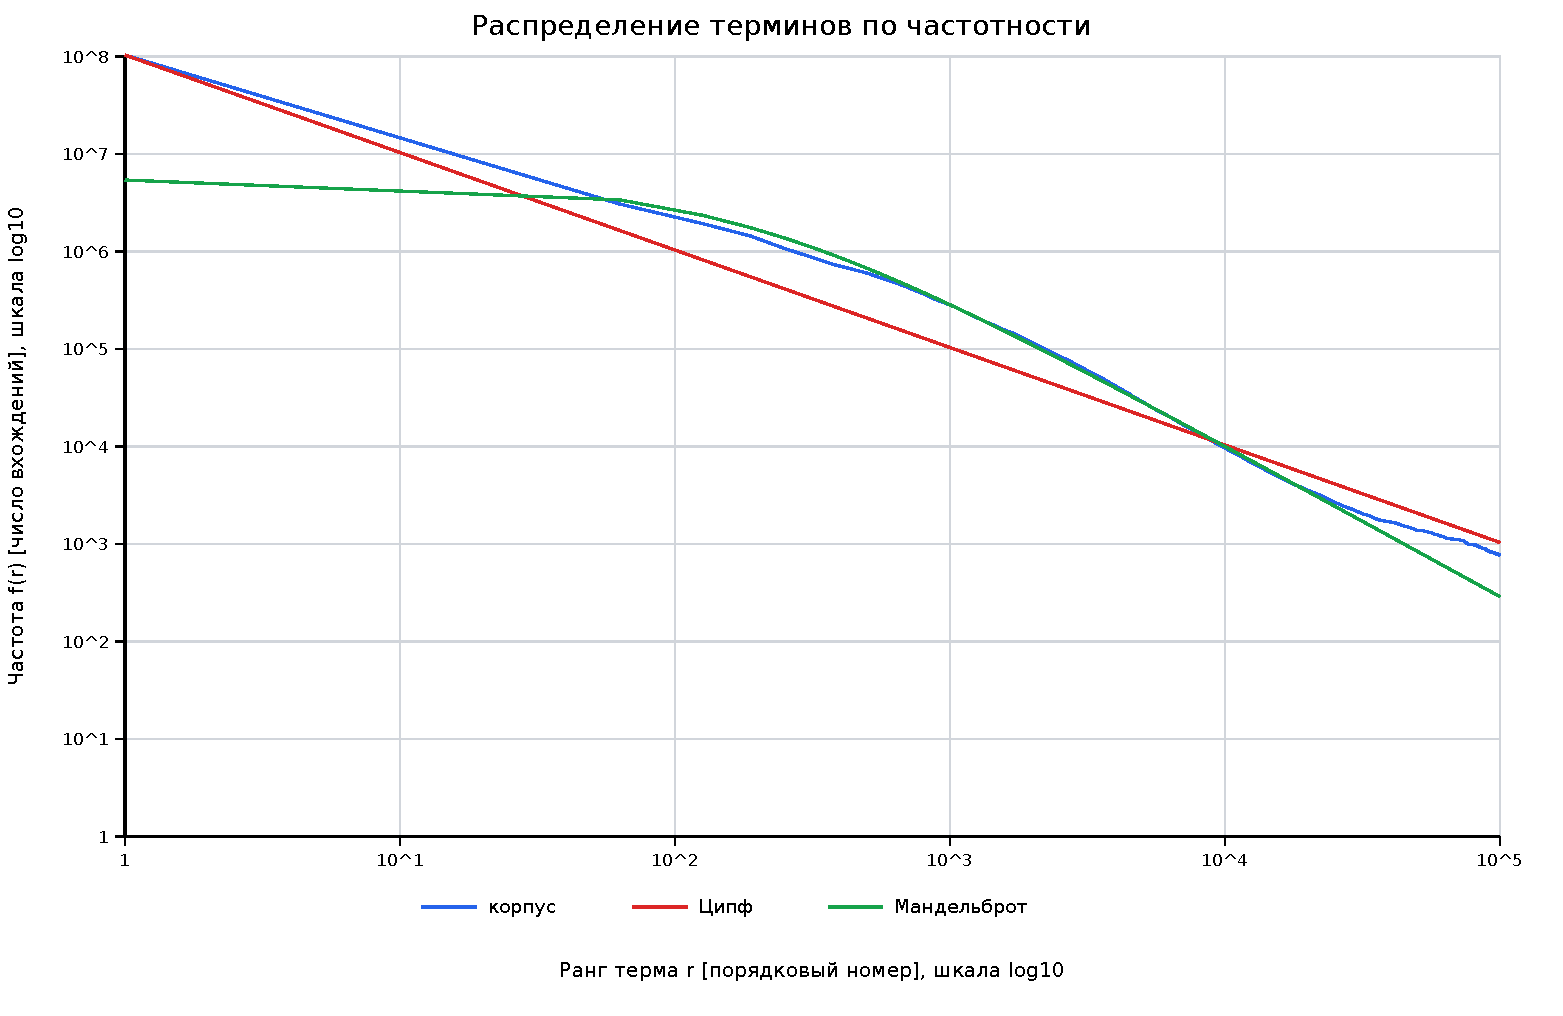
\includegraphics[width=\textwidth]{../images/search_system_zipf.pdf}
\caption{Частоты лемм технического корпуса и теоретические модели. Ранг и число вхождений
показаны в логарифмических шкалах.}
\end{figure}

\partlabel{Выполнение и результаты}
Частоты подсчитываются по принятым документам, отдельно до и после
лемматизации. На графике показано распределение лемм: первые 100\,000 термов; подбор модели
выполняется по первым 10\,000. Получены значения
$C=1{,}6337\cdot10^{10}$, $b=174{,}753$, $s=1{,}55083$;
RMSE логарифмов частот равна 0,09018. Это ошибка выбранной аппроксимации
на участке подбора, а не показатель качества поиска.

Самый частый токен - \code{the}, 103\,167\,741 вхождение.
После лемматизации формы глагола объединяются в \code{be}, частота которого
составляет 41\,093\,445. Наряду с обычными служебными словами высокие частоты
имеют технические обозначения и остатки шаблонного содержимого. Поэтому
наблюдаемое распределение нельзя объяснять только свойствами обычной прозы.

\partlabel{Проверки и вывод}
Проверяются порядок рангов, неотрицательные частоты, корректность подбора
модели и подписи осей графика. Сохраненные JSON-данные позволяют восстановить
численные параметры независимо от изображения. Характерное убывание частот
наблюдается, но идеального совпадения с $C/r$ нет. Отклонения объясняются
смешением жанров, программным кодом, числовыми термами и шумом извлечения.
Улучшать соответствие графику искусственным удалением неудобных слов не следует:
важнее использовать распределение как средство диагностики корпуса.

\labsection{6}{Оценка качества поиска}

\partlabel{Задание и организация эксперимента}
Цель эксперимента - проверить полезность первых результатов TF-IDF на
реальных информационных потребностях. Я зафиксировал 30 англоязычных запросов
по программированию, базам данных, безопасности, машинному обучению и смежным
техническим темам. Для каждого запроса записано намерение пользователя.
В качестве альтернатив использованы поиски Wikipedia, Microsoft Learn
и arXiv. Для оценки берутся первые пять результатов. arXiv добавлен отдельным
этапом через Atom API: исходные термы соединены AND, задана сортировка
по релевантности, получено до десяти результатов на запрос. У двух запросов
выдача пустая, еще у трех короче пяти; они остаются в среднем по 30 запросам.

Индекс во время эксперимента не перестраивался: в нем 993\,923 документа,
19\,009\,884 терма и 524\,192\,226 пар «терм - документ». В
\code{quality_evaluation} сохранены запросы, выдачи, тексты для оценки,
оценки с обоснованиями, таблицы метрик и контрольные суммы снимка. Повторный
расчет по сохраненным данным не требует повторного обращения к сайтам.

Попытки использовать общие веб-поисковики ограничивались страницами согласия,
CAPTCHA и неполными ответами. Неполная выдача Bing оставлена как дополнительное
наблюдение и не включена в основную сравнительную таблицу. Выбор альтернатив
следует учитывать при интерпретации результатов: они работают по другим
наборам документов и ориентированы на свои источники.

\partlabel{Разметка и определения метрик}
Общий пул содержит 608 пар «запрос - документ», соответствующих 589 уникальным
документам. Каждой паре присваивается оценка: 0 - документ не отвечает
намерению, 1 - затрагивает тему лишь косвенно, 2 - дает полезную часть ответа,
3 - прямо и содержательно отвечает на запрос. В пуле получено 170 нулей,
174 единицы, 199 двоек и 65 троек.

Разметка является \textbf{пилотной}: первичные оценки выставлены языковой
моделью по сохраненному содержимому и фрагментам; для 131 новой статьи arXiv
использованы заголовки и аннотации API. Это не независимый эталон
человеческой разметки. Оценки и причины сохранены для последующей проверки
человеком; результаты не следует представлять как окончательно доказанное
качество системы.

Пусть $g_i\in\{0,1,2,3\}$ - оценка документа на позиции $i$, а $k$ - глубина
выдачи. В эксперименте релевантными для точности считаются оценки не ниже 2:
\[
 P@k=\frac{1}{k}\sum_{i=1}^k [g_i\geq2],\qquad
 DCG@k=\sum_{i=1}^k\frac{2^{g_i}-1}{\log_2(i+1)}.
\]
$P@k$ показывает долю полезных результатов, а DCG учитывает степень
полезности и понижает вклад поздних позиций. Нормированная метрика
$NDCG@k=DCG@k/IDCG@k$ сравнивает выдачу с идеальным порядком оценок из
собранного пула. При $IDCG=0$ результат принимается равным нулю. Это идеал
среди оцененных документов, а не среди всех страниц интернета.

Для ERR вводится условная вероятность удовлетворения
$R_i=(2^{g_i}-1)/8$. Тогда
\[
 ERR@k=\sum_{i=1}^k\frac{R_i}{i}\prod_{j=1}^{i-1}(1-R_j).
\]
Метрика моделирует просмотр сверху вниз: после полезного ответа вероятность
продолжения уменьшается. Значения $R_i$ задаются шкалой оценок и не измерялись
на настоящих пользователях. Все четыре метрики усредняются по 30 запросам
с одинаковым весом запроса.

\begin{table}[htbp]\centering
\caption{Средние метрики пилотной оценки, глубина @5}
\begin{tabularx}{\textwidth}{Yrrrr}
\toprule
Система & P@5 & DCG@5 & NDCG@5 & ERR@5\\
\midrule
TF-IDF & 0,3733 & 5,6645 & 0,3710 & 0,4212\\
Wikipedia & 0,5533 & 9,8162 & 0,6512 & 0,7238\\
Microsoft Learn & 0,1733 & 3,0337 & 0,1990 & 0,2237\\
arXiv & 0,6533 & 6,9938 & 0,4751 & 0,4806\\
\bottomrule
\end{tabularx}
\end{table}

\begin{figure}[!ht]\centering
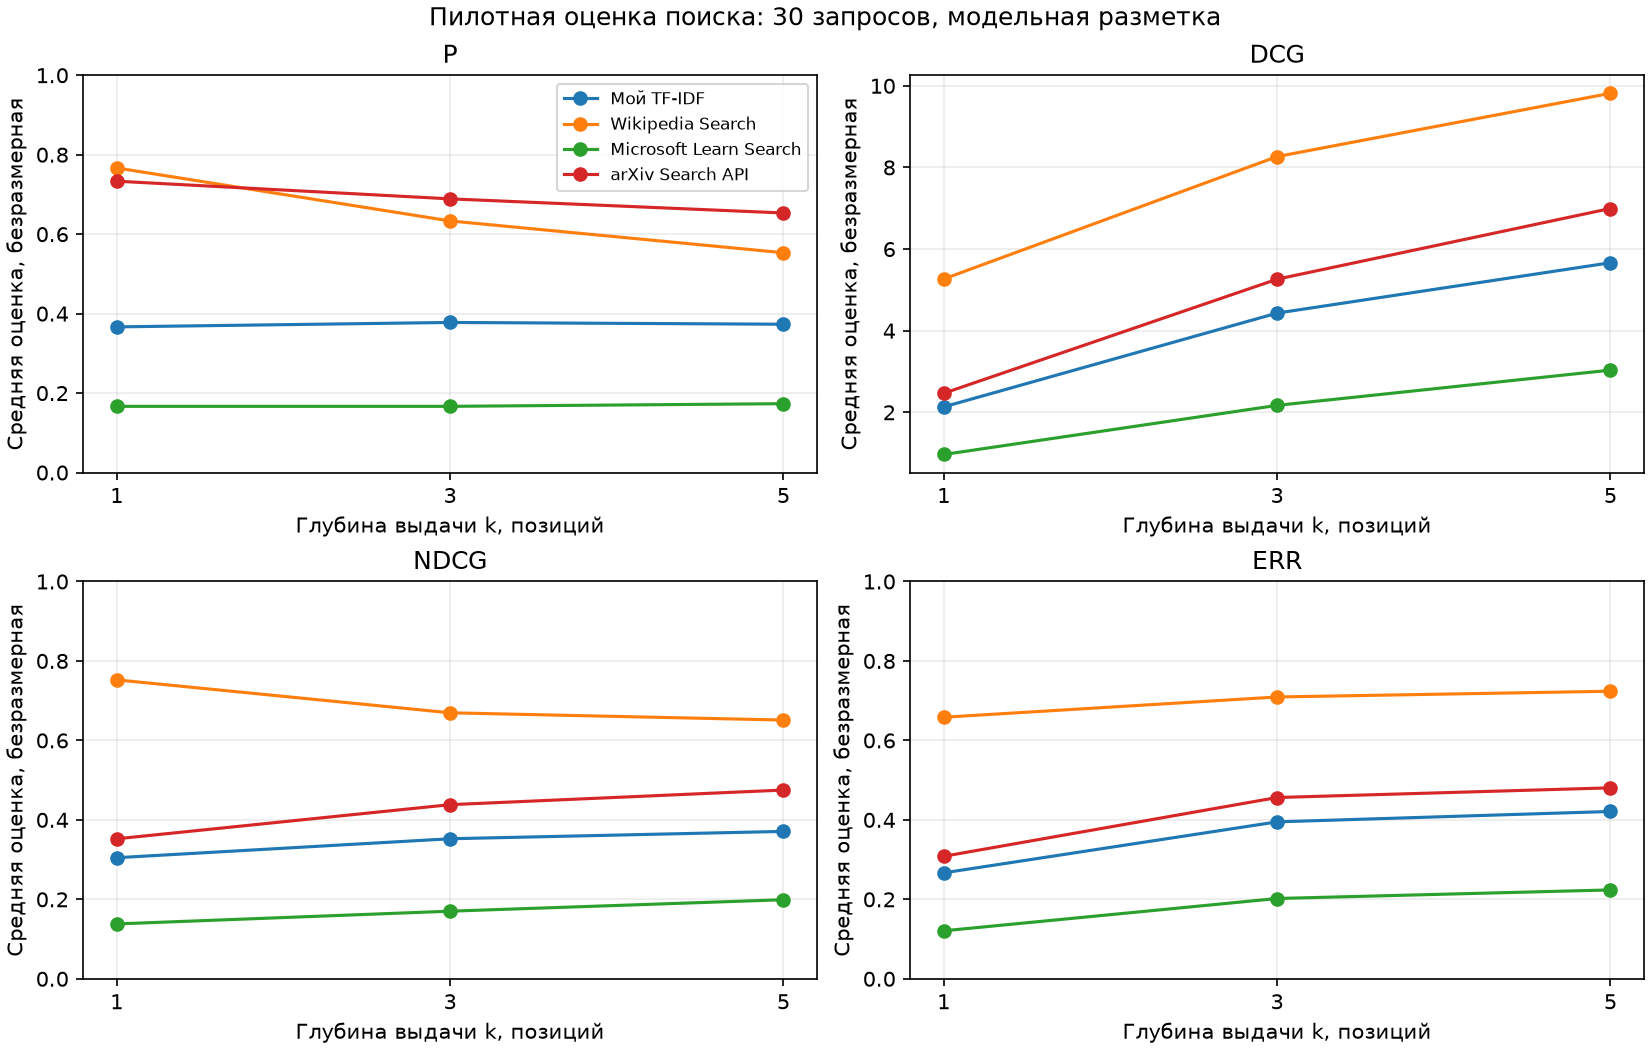
\includegraphics[width=\textwidth]{../../quality_evaluation/metrics.png}
\caption{Средние P, DCG, NDCG и ERR на глубинах @1, @3 и @5.
Первичная разметка модельная; результаты требуют проверки человеком.}
\end{figure}

\partlabel{Разбор результатов и проверки}
Для TF-IDF получены $P@1=0{,}3667$, $NDCG@1=0{,}3048$ и
$P@3=0{,}3778$, $NDCG@3=0{,}3525$. Система удачно отвечает на часть
узких запросов: для retrieval augmented generation получены
$P@5=1{,}0$ и $NDCG@5\approx0{,}842$. На запросе о конфиденциальности
federated learning первые результаты уходят в федеративную аутентификацию,
и $P@5=0$. При этом подходящий материал присутствует в индексе, что указывает
именно на проблему выбора результатов. Запросы о transformer attention
также страдают от неоднозначности терминов.

Покрытие альтернатив корпусом различается: среди 150 позиций Wikipedia
142 соответствуют документам индекса, а среди 150 позиций Microsoft Learn -
62; из 131 позиции arXiv в индексе присутствуют 9. Поэтому различие метрик
связано и с ранжированием, и с покрытием. arXiv нашел прямую научную работу
о Variable Byte, которой не было в исходном пуле. При расширении пула прежние
выдачи и оценки сохранены, но NDCG пересчитана по новому общему идеалу;
изменение ее значения не означает изменения алгоритма.
Нельзя делать вывод о превосходстве алгоритма только по этой таблице.
Формулы, граничные случаи и разбор ответов проверяются 19 Python-тестами;
все они прошли.

\partlabel{Вывод}
Эксперимент выявил как удачные тематические совпадения, так и ошибки смысла
у многозначных терминов. Он дает воспроизводимую исходную точку для следующего
сравнения, но не доказывает рост метрик после отдельного улучшения:
контролируемого измерения «до и после» здесь нет. Следующие обоснованные шаги -
проверка разметки человеком и разбор ошибочных запросов с учетом покрытия
корпуса, а не подгонка оценок под ожидаемый результат.

\labsection{7}{Булев индекс}

\partlabel{Задание и входные данные}
Обратный индекс должен позволять быстро получить документы, содержащие заданный
терм. Его входом служит коллекция \code{document_terms}: для каждого принятого
документа в ней хранятся термы и их частоты. Это прямое представление
«документ - термы». Построитель разворачивает его в представление
«терм - упорядоченный список документов».

Индекс строится по леммам. Внутренние \code{docID} присваиваются подряд,
от 0 до $N-1$, где $N$ - число принятых документов. Таблица соответствия
12-байтовому MongoDB ObjectId сохраняется отдельно. Таким образом,
постинг содержит компактный номер документа, а не длинный строковый URL.

\partlabel{Построение на внешней памяти}
Все пары корпуса не загружаются одновременно в оперативную память.
Обрабатываются блоки по 500\,000 пар «терм - документ» с частотой.
Блок сортируется и записывается во временный файл. Затем выполняется
многопутевое слияние; при большом числе файлов используются промежуточные
проходы с ограниченным числом одновременно открытых входов. Одинаковые термы
собираются вместе, документы внутри их списков идут по возрастанию \code{docID}.

Такой способ переносит основной объем данных на диск. Память определяется
размером блока и буферами слияния, а не всем числом вхождений в корпусе.
Цена подхода - дополнительный дисковый ввод-вывод и временное место для блоков.
Частота хранится вместе с документом, поэтому один основной индекс пригоден
и для булевых операций, и для TF-IDF.

\begin{table}[htbp]\centering
\caption{Назначение файлов основного индекса, версия 4}
\begin{tabularx}{\textwidth}{lY}
\toprule
Файл & Содержимое и использование\\
\midrule
\code{lexicon.bin} & Заголовок и записи термов: смещения строк и списков,
длина терма, число документов $df$.\\
\code{terms.bin} & Подряд записанные UTF-8-байты термов в словарном порядке.\\
\code{postings.bin} & Сжатые пары: разность \code{docID} и частота терма.\\
\code{documents.bin} & Соответствие внутреннего \code{docID} MongoDB ObjectId.\\
\code{norms.bin} & Предвычисленные длины векторов документов для TF-IDF.\\
\code{skips.bin} & Разреженные указатели для ускорения пересечения списков.\\
\bottomrule
\end{tabularx}
\end{table}

\partlabel{Формат и результат}
Заголовок \code{lexicon.bin} занимает 32 байта и содержит сигнатуру,
версию, число документов, термов и постингов. Одна запись словаря занимает
24 байта: два 64-битных смещения и два 32-битных поля длины терма и $df$.
Границы строк не определяются нулевыми символами: они берутся из записи словаря.
Числа сохранены в little-endian представлении используемой платформы x86-64.
Это явное ограничение переносимости текущего формата.

Итоговый индекс содержит 993\,923 документа, 19\,009\,884 терма
и 524\,192\,226 пар «терм - документ». Суммарный размер шести файлов
равен 2\,066\,772\,566 байтам ($1{,}925\GiB$). При поиске терм
находится двоичным поиском в упорядоченном словаре. По его смещению читается
соответствующий список; последовательное чтение всего \code{postings.bin}
для одного запроса не требуется.

\partlabel{Проверки и вывод}
Тестируются пустой и малый корпус, одинаковые термы в разных документах,
подсчет частот, границы блоков, объединение файлов, отображение \code{docID},
заголовки и поврежденные данные. Поиск проверяется на искусственных индексах
с заранее известными списками. Индекс пригоден для большого корпуса,
поскольку строится блоками; при этом он является статическим снимком.
После существенного изменения текстов и правил обработки требуется
согласованное перестроение, а не простая дозапись произвольных байтов в файл.

\labsection{8}{Булев поиск}

\partlabel{Задание и разбор запроса}
Булев поиск возвращает документы, удовлетворяющие логическому выражению
над термами. Поддерживаются операции \code{AND}, \code{OR}, \code{NOT}
и скобки. Запрос читается из стандартного ввода, результаты выводятся
в стандартный вывод. Найденные документы показываются с заголовком и URL;
метаданные восстанавливаются через таблицу ObjectId и MongoDB.

Сначала лексер выделяет термы, операторы и скобки. Затем рекурсивный спуск
разбирает выражение с приоритетами: \code{NOT} выше \code{AND},
\code{AND} выше \code{OR}. Скобки изменяют порядок вычисления.
Лингвистическая нормализация применяется к термам, но не превращает ключевые
операторы в обычные поисковые слова.

\begin{lstlisting}
cloud AND (security OR database)
\end{lstlisting}

Для этого запроса сначала вычисляется объединение списков \code{security}
и \code{database}, затем пересечение с \code{cloud}. Рекурсивные вызовы
соответствуют вложенности выражения. Некорректные скобки, отсутствующий операнд
и лишние токены дают ошибку запроса, а не произвольную частичную выдачу.

\partlabel{Вычисление над списками}
Список каждого нужного терма декодируется отдельно. Для \code{AND}
используется пересечение двух отсортированных списков: сравниваются текущие
номера, меньший указатель продвигается, одинаковый номер добавляется в ответ.
Для \code{OR} выполняется слияние без повторов. \code{NOT} строит дополнение
относительно всех внутренних \code{docID} текущего индекса.

Если длины двух списков равны $a$ и $b$, линейное пересечение и объединение
имеют сложность $O(a+b)$. Дополнение может потребовать $O(N)$, где $N$ - число
индексированных документов. Поэтому запрос с одним частым термом или большим
отрицанием может создавать крупный промежуточный ответ. Ограничение выдачи
в 20 результатов сокращает показ пользователю, но не означает, что логическое
выражение проверяется только на 20 документах.

\partlabel{Пример и проверки}
Пусть списки равны:
\begin{lstlisting}
cloud:    [0, 2, 5, 8]
security: [2, 4, 8]
database: [1, 5]
security OR database -> [1, 2, 4, 5, 8]
cloud AND (...)      -> [2, 5, 8]
\end{lstlisting}

Тесты охватывают таблицы истинности, приоритеты, вложенные скобки, двойное
отрицание, неизвестные термы, пустые результаты, отсутствие дублей,
нормализацию специальных имен и ошибки синтаксиса. Одинаковые запросы
проверяются с включенными и выключенными прыжками; результат должен совпадать.

\partlabel{Вывод}
Булев поиск удобен, когда пользователь может точно сформулировать обязательные
и альтернативные термы. Он не оценивает степень полезности: все найденные
документы удовлетворяют выражению, но не ранжируются по смыслу. Для свободного
текстового запроса применяется отдельный TF-IDF-поиск на том же основном
индексе. В настоящем отчете рассматривается реализованный консольный способ
взаимодействия.

\labsection{10}{Цитатный поиск и координатный индекс}

\partlabel{Задание и необходимость координат}
Цитатный поиск должен находить документы с заданной последовательностью слов.
Обычный обратный индекс отвечает только на вопрос о присутствии термов:
он не различает «cloud security» и «security cloud». Для проверки порядка
нужно дополнительно хранить позиции каждого терма в документе.

Входом служат принятые тексты из \code{processed_documents}, поскольку
прямой индекс частот уже потерял исходную последовательность. Тексты повторно
проходят те же токенизатор и лемматизатор. Таблица внутренних \code{docID}
берется из основного индекса, чтобы результаты двух индексов ссылались
на одинаковые MongoDB-документы.

\partlabel{Построение и формат}
Генерируются тройки «терм - документ - позиция». Внешняя сортировка выполняется
блоками по 500\,000 отдельных вхождений, затем блоки сливаются с ограниченным
числом одновременно открытых файлов. Здесь объем входа больше, чем у обычного
индекса: десять повторений слова дают десять позиций, а не одну пару с частотой.

Файл \code{coordinate_lexicon.bin} содержит 40-байтовый заголовок
и 32-байтовые записи термов. В заголовке указаны версия 1, число документов,
термов, пар и позиций. UTF-8-строки лежат в \code{coordinate_terms.bin},
а списки документов и позиций - в \code{coordinates.bin}. Используются
разности номеров и позиций с кодированием Variable Byte.

\partlabel{Алгоритм поиска}
Запрос нормализуется в последовательность $t_0,t_1,\ldots,t_{m-1}$,
где $m$ - число термов. Сначала пересекаются списки документов этих термов.
В каждом документе-кандидате проверяется наличие стартовой позиции $p$,
для которой термы стоят на позициях $p,p+1,\ldots,p+m-1$.
Повторяющиеся термы требуют разных последовательных позиций.

\begin{lstlisting}
Document: cloud security improves cloud security
cloud:    [0, 3]
security: [1, 4]
Query:    cloud security
Starts:   [0, 3]
\end{lstlisting}

Поиск является точным по последовательности \emph{нормализованных токенов},
а не по исходным байтам HTML. Регистр, часть пунктуации и различия словоформ
уже устранены. Это необходимо оговаривать, чтобы не обещать буквальное
совпадение исходной цитаты вместе со всеми знаками оформления.

\partlabel{Результаты, проверки и вывод}
Координатный индекс содержит 2\,205\,065\,484 позиции
и 524\,192\,226 пар «терм - документ». Три файла занимают
5\,296\,876\,623 байта ($4{,}933\GiB$). Основной поток координат
занимает 4\,409\,828\,968 байт; словарь и строки занимают оставшуюся часть.
Большой объем и промежуточные слияния объясняют длительность построения:
завершение чтения документов еще не означает завершения слияния блоков.

Тестируются правильный и обратный порядок, пропущенные слова, фраза из одного
терма, повтор одного слова, несколько вхождений фразы и отсутствующий терм.
Отдельный координатный индекс сохраняет компактность обычного булева поиска,
но увеличивает дисковое место и требует согласования снимков двух индексов.

\labsection{11}{Сжатие индекса}

\partlabel{Задание и представление чисел}
Необходимо уменьшить размер списков без потери документов, частот и позиций.
Основной прием состоит из двух частей: перехода к разностям отсортированных
чисел и кодирования Variable Byte. Если номера документов равны
$[3,10,130]$, записываются разности $[3,7,120]$. Первый номер считается
относительно нуля. Последовательное суммирование восстанавливает исходные
номера без потерь.

Variable Byte разбивает неотрицательное целое число на группы по 7 значащих
битов. В каждом байте младшие 7 бит хранят данные, а старший бит является
признаком последнего байта числа. В данной реализации старший бит равен 1
\emph{у последнего} байта. Группы записываются от старшей к младшей.
Поэтому числа от 0 до 127 занимают один байт, более крупные - несколько.

\begin{lstlisting}
130 = 1 * 128 + 2
Data groups: 0000001  0000010
Bytes:       00000001 10000010 = 0x01 0x82
Decode:      1 * 128 + 2 = 130
\end{lstlisting}

Кодирование применяется и к частоте терма. В координатном индексе дополнительно
кодируются разности позиций внутри документа. Декодер ограничивает длину
32-битного числа пятью байтами, проверяет переполнение и отсутствие
завершающего байта. Таким образом, поврежденные данные не должны незаметно
превращаться в другое корректное число.

\partlabel{Измерение степени сжатия}
Базовое представление обычного постинга содержит два \code{uint32_t}:
номер документа и частоту, всего 8 байт. При $M=524\,192\,226$ постингах
базовый объем равен $8M=4\,193\,537\,808$ байт. Реальный
\code{postings.bin} занимает $B=1\,195\,110\,523$ байта. Экономия:
\[
 E=\left(1-\frac{B}{8M}\right)\cdot100\,\%=71{,}50\,\%.
\]
Это сокращение именно потока постингов, а не всего индекса с его словарем,
таблицей документов, нормами и прыжками. В среднем на пару приходится
около 2,28 байта вместо 8.

Для координат базовая оценка равна $8M+4T$, где $T=2\,205\,065\,484$ -
число позиций. Получается 13\,013\,799\,744 байта. Сжатый поток координат
занимает 4\,409\,828\,968 байт; экономия относительно этой базы -
66,11\,\%. В эту оценку также не включены словарные файлы.

\partlabel{Проверки и вывод}
Проверяются числа 0, 127, 128, границы следующих длин, максимальное
\code{uint32_t}, последовательность нескольких чисел, оборванные данные
и переполнение. Для списков проверяется восстановление исходных номеров
и частот. Сжатие без потерь сохраняет состав выдачи при правильном декодировании;
проверки эквивалентности подтверждают это на тестовых данных. Отдельного
повторного эксперимента всех метрик качества на несжатом полном индексе
не выполнялось.

Подход хорошо подходит малым разностям, но требует последовательного
декодирования списка. Для отдельного терма читается его собственный поток,
а не весь файл индекса. Прямой переход в произвольный байт без знания границы
числа и предыдущего абсолютного \code{docID} невозможен.

\labsection{12}{Ускорение: прыжки по индексу}

\partlabel{Задание и алгоритм}
Прыжки ускоряют пересечение длинных списков, позволяя пропускать отрезки,
которые заведомо не содержат нужного номера документа. Для списка длины $P$
шаг разреженной разметки выбирается примерно равным $\lfloor\sqrt{P}\rfloor$.
Здесь $P$ - количество документов, содержащих конкретный терм, а не общий
размер корпуса. Для списков короче 16 постингов указатели не создаются.

В \code{skips.bin} для терма сохраняется диапазон его указателей. Каждый
указатель содержит \code{posting_index} - позицию цели внутри декодированного
списка, и \code{document_id} - абсолютный номер документа в этой позиции.
Источник перехода определяется текущей позицией алгоритма; отдельное поле
«откуда» в записи не требуется.

Если текущий документ одного списка меньше текущего документа другого,
проверяется допустимая цель прыжка. Перейти можно, только когда номер цели
не больше сравниваемого номера другого списка. Например, при поиске номера
300 цель 250 безопасна: пропущенные номера тоже меньше 300. Цель 350
не подходит, поскольку при таком переходе можно пропустить совпадение 300.

В данной реализации прыжки применяются после декодирования списков в память.
Они уменьшают работу пересечения, но не являются переходами по сжатым байтам
\code{postings.bin}. Времени на чтение и декодирование терма они сами
по себе не устраняют.

\partlabel{Сравнительный эксперимент}
Отдельный Google Test-исполняемый файл сравнивает одинаковые операции с прыжками
и без них. Используются синтетические списки до 200\,000 элементов;
сверяется идентичность результата, считаются сравнения и берется медиана
11 повторений. Измеряется участок пересечения уже подготовленных списков,
а не полный запрос с MongoDB и дисковым чтением.

\begin{table}[htbp]\centering
\caption{Пересечение списков: измеренное время и число сравнений}
\begin{tabularx}{\textwidth}{Yrrrr}
\toprule
Сценарий & \multicolumn{2}{c}{Медиана, мкс} & \multicolumn{2}{c}{Сравнения}\\
 & Линейно & Прыжки & Линейно & Прыжки\\
\midrule
Совпадение в конце & 225,499 & 0,601 & 200\,000 & 192\\
Разреженные цели & 191,846 & 14,257 & 200\,000 & 8\,689\\
Чередующиеся номера & 180,704 & 358,713 & 199\,999 & 199\,999\\
\bottomrule
\end{tabularx}
\end{table}

В первом сценарии один прыжок заменяет 199\,809 последовательных шагов,
число сравнений сокращается на 99,90\,\%. Во втором выполняется 40 прыжков,
экономия сравнений составляет 95,66\,\%. В третьем полезных переходов нет,
а проверки указателей добавляют затраты: наблюдается замедление. Приведенное
время зависит от машины и не является универсальным обещанием ускорения.

\partlabel{Проверки и вывод}
Тестируются границы указателей, равенство номера цели текущей цели другого
списка, отсутствие подходящего перехода и одинаковый ответ обоих алгоритмов.
Размер \code{skips.bin} текущего индекса равен 116\,814\,976 байтам,
то есть ускорение требует дополнительного места. Прыжки полезны при
неравномерно пересекающихся длинных списках; для плотно чередующихся списков
они не сокращают число сравнений. Это ограничение подтверждено экспериментом,
а не скрыто за единственным удачным примером.

\labsection{13}{TF-IDF}

\partlabel{Задание и связь с индексом}
Ранжирование должно упорядочить найденные документы по степени лексического
соответствия свободному запросу. TF-IDF повышает вес частого в данном документе
терма и уменьшает влияние термов, встречающихся почти повсюду. Используется
тот же основной обратный индекс: $tf_{t,d}$ читается из постинга, а
$df_t$ - из записи словаря. $N$ берется из заголовка индекса.

Здесь $tf_{t,d}$ - число вхождений терма $t$ в документ $d$, $df_t$ - число
документов с этим термом, $N$ - число документов индекса. Выбрана схема
SMART \code{lnc.ltc}: логарифмический TF и нормирование документа;
логарифмический TF, IDF и нормирование запроса.

\partlabel{Формулы и выполнение запроса}
Для присутствующего в документе терма вычисляется
$u_{t,d}=1+\log_{10}tf_{t,d}$. Затем
\[
 L_d=\sqrt{\sum_t u_{t,d}^{\,2}},\qquad w_{t,d}=u_{t,d}/L_d.
\]
В сумме участвуют все термы документа; $L_d$ заранее сохраняется в
\code{norms.bin}. IDF в вес документа не включается. Для запроса с частотой
$tf_{t,q}$ используются
\[
 v_{t,q}=(1+\log_{10}tf_{t,q})\log_{10}(N/df_t),\qquad
 L_q=\sqrt{\sum_t v_{t,q}^{\,2}},\qquad w_{t,q}=v_{t,q}/L_q.
\]
Если длина вектора равна нулю, деление не выполняется. Отсутствующий
в индексе терм не создает кандидатов. Термы с $df_t=N$ получают нулевой IDF.
Косинусная оценка документа равна
\[
 score(d,q)=\sum_{t\in d\cap q}w_{t,d}w_{t,q}.
\]
Таким образом, высокий счет требует совпадений с запросом; документ без
единого совпадающего терма в ранжирование не попадает. Совпадение всех слов
не обязательно, в отличие от булевого \code{AND}.

После нормализации запроса читаются списки только его термов. Вклад каждого
постинга накапливается в массиве \code{scores}, индексом которого служит
\code{docID}. Дополнительный список \code{touched_documents} запоминает
документы с ненулевым вкладом, чтобы не обходить весь массив при сборке ответа.
Кандидаты полностью сортируются по убыванию оценки, при равенстве - по
\code{docID}; затем применяется лимит выдачи. Из MongoDB берутся заголовки и URL уже выбранных
документов; вычисление TF-IDF не выполняет полнотекстовый поиск по MongoDB.

Пусть $V$ - размер словаря, $m$ - число различных термов запроса,
$S=\sum_{t\in q}df_t$ - число просмотренных постингов, $C$ - число кандидатов,
$N$ - число документов индекса. Обнуление массива оценок занимает $O(N)$,
а полная оценка основной работы равна
$O(N+m\log V+S+C\log C)$, без учета стоимости нормализации и дискового чтения.
Память включает $O(N)$ оценок, кандидатов и текущий загруженный список.
Для данного снимка массив \code{double} занимает около 7,58 МиБ.
Прямое обращение по номеру документа упрощает реализацию и не требует
хеш-таблицы, но обнуление и полная сортировка остаются затратами каждого запроса.

\partlabel{Результат и проверки}
Ранжирование работает на индексе из 993\,923 документов. Лимит выдачи в
конфигурации равен 20. Корректность проверяется на небольших искусственных
индексах: веса рассчитываются вручную и сопоставляются с результатами
программы. Проверяются повтор слова в запросе, частый и редкий терм,
неизвестные слова, нулевой вектор, нормирование документов разной длины,
ограничение количества результатов и согласованность метаданных.
Эти тесты не зависят от наполнения пользовательской MongoDB.

\partlabel{Вывод}
TF-IDF дает объяснимое ранжирование и повторно использует частоты булева
индекса. Косинусная оценка не является вероятностью релевантности и не понимает
смысл многозначных терминов. Эксперимент раздела 6 показывает это на конкретных
запросах. Нормирование уменьшает простое преимущество длинного документа,
но не устраняет шум, неоднозначность и различия жанров корпуса.

\labsection{17}{Автотесты}

\partlabel{Задание и план}
Тесты должны проверять корректность компонентов независимо от текущего
состояния большого корпуса. Для C++ используется Google Test с запуском
через CTest. Для робота и расчетов метрик применяется pytest. Основной принцип
плана - проверять наблюдаемое поведение и граничные случаи, а не только
успешный запуск программы.

\begin{longtable}{p{34mm}p{\dimexpr\textwidth-34mm-4\tabcolsep\relax}}
\caption{Основные группы проверок}\\
\toprule
Компонент & Проверяемое поведение\\
\midrule
\endfirsthead
\multicolumn{2}{r}{Продолжение таблицы \thetable}\\
\toprule
Компонент & Проверяемое поведение\\
\midrule
\endhead
Токенизатор & Unicode, ошибочные байты, пробелы и пунктуация, длины,
технические конструкции и их повторения.\\
Лемматизатор & Словарные формы, исключения, технические переопределения,
неизвестные слова, неоднозначность.\\
Основной индекс & Блоки сортировки, частоты, порядок документов, бинарные
форматы, кодирование и декодирование.\\
Булев поиск & Операции, приоритеты, рекурсия, ошибки запроса, прыжки,
совпадение с эталонным пересечением.\\
TF-IDF & Численные веса, нормы, порядок результатов, редкость терма,
пустые запросы и выбор лучших результатов.\\
Цитатный поиск & Координаты, порядок, соседство, повтор термов, несколько
вхождений и отсутствующие фразы.\\
Робот & Очереди, контрольные точки, обновление, обработка сетевых ответов,
конфликты уникальности и ограничения.\\
Оценка качества & Формулы P, DCG, NDCG, ERR, шкала оценок и крайние случаи.\\
\bottomrule
\end{longtable}

\partlabel{Выполнение и результат}
Контрольный прогон дал 207 успешных CTest-проверок из 207. По текущим меткам
CTest это 201 unit-проверка, три сравнительных performance-проверки и три
проверки с меткой integration. Последние проверяют отдельные свойства
обработки и отчетных данных; это не полный сквозной тест всей системы
с новой MongoDB и реальным обходом внешних сайтов.

Отдельно выполнены 64 теста робота и 19 тестов оценки качества:
все 83 Python-проверки прошли. Три сравнительных теста прыжков проверяют
равенство ответов и печатают измерения, приведенные в разделе 12.
Они уже входят в число 207 и не прибавляются к нему повторно.

\begin{lstlisting}
ctest --test-dir .build --output-on-failure
100% tests passed, 0 tests failed out of 207

uv run pytest tests/crawler/test_crawler.py quality_evaluation/test_metrics.py -q
83 passed
\end{lstlisting}

\partlabel{Вывод}
Малые детерминированные примеры позволяют проверять структуру индекса и
арифметику независимо от пользовательской базы. Прогоны подтверждают
проверенные сценарии, но не заменяют оценку полезности выдачи и испытание
всех сетевых отказов. Полезное дальнейшее дополнение - полный сквозной
прогон на отдельном небольшом фиксированном корпусе с проверкой всех
сохраненных результатов.

\clearpage
\section*{Сборка и последовательность запуска}
\addcontentsline{toc}{section}{Сборка и последовательность запуска}

Команды выполняются из корня проекта в Linux или WSL. MongoDB запускается
через Docker Compose на порту 27017, Python-зависимости устанавливаются через uv.

\begin{lstlisting}
sudo apt install build-essential cmake libmongoc-dev libbson-dev libxml2-dev
uv sync
docker compose up -d
cmake -S . -B .build -DCMAKE_BUILD_TYPE=Release
cmake --build .build --parallel
\end{lstlisting}

Начальное исследование источников открывается в Jupyter:
\begin{lstlisting}
uv run jupyter notebook notebooks
\end{lstlisting}
Для построения системы с нуля
последовательно выполняются загрузка, лингвистическая обработка и индексация:

\begin{lstlisting}
uv run python src/crawler/main.py configs/crawler.yaml
./.build/linguistics configs/linguistics.yaml
./.build/boolean_index configs/boolean_index.yaml
./.build/positional_index configs/positional_index.yaml
\end{lstlisting}

Основной индекс строится раньше координатного, поскольку последний использует
его таблицу документов. При наличии готовых индексов загрузку и построение
повторять для демонстрации не нужно.

\begin{lstlisting}
printf 'cloud AND (security OR database)\n' | ./.build/boolean_search configs/search.yaml
printf 'retrieval augmented generation\n' | ./.build/tfidf_search configs/search.yaml
printf 'machine learning\n' | ./.build/phrase_search configs/search.yaml
\end{lstlisting}

Для интерактивного ввода программа запускается без \code{printf}.
Проверки и расчет сохраненного эксперимента:

\begin{lstlisting}
ctest --test-dir .build --output-on-failure
./.build/boolean_search_comparison_tests
uv run pytest tests/crawler/test_crawler.py quality_evaluation/test_metrics.py -q
uv run python quality_evaluation/evaluate.py
\end{lstlisting}

Пути внутри конфигураций задаются относительно соответствующего YAML-файла.
Исходные тексты и конфигурации прилагаются к отчету; корпус и индексы
передаются отдельно из-за их размера.

\clearpage
\section*{Общие выводы}
\addcontentsline{toc}{section}{Общие выводы}

Создана система, в которой оригиналы документов сохраняются независимо
от правил обработки, а поиск работает по дисковым индексам. Загрузку можно
продолжать после остановки, тексты - переразбирать из MongoDB, индекс - строить
внешней сортировкой. Основной индекс обслуживает булев поиск и TF-IDF,
координатный добавляет проверку порядка термов.

На снимке из 993\,923 принятых документов размер основного индекса составляет
1,925 ГиБ, координатного - 4,933 ГиБ. Экономия потока обычных постингов
относительно пар 32-битных чисел равна 71,50\,\%. Прыжки существенно
уменьшают число сравнений в подходящих сценариях, но могут замедлять
пересечение, когда безопасных переходов нет. Эти результаты относятся
к конкретному формату и измеренным сценариям.

Ограничения связаны с тематическим дрейфом категорий Wikipedia, артефактами
HTML и отсутствием контекстного понимания слов у лемматизации и TF-IDF.
Пилотная оценка показывает, что лексическое совпадение не гарантирует
полезной выдачи. Приоритет дальнейшей работы - проверка разметки человеком,
очистка источников шума и сравнение ранжирования на фиксированных запросах.

\section*{Источники и материалы}
\addcontentsline{toc}{section}{Источники и материалы}
\begin{enumerate}\setlength{\itemsep}{2pt}\setlength{\parskip}{0pt}
\item Курс «Информационный поиск»: требования и перечень работ.\\
\url{https://github.com/toshunster/MAI-IR}
\item TeX-шаблон отчета преподавателя.\\
\url{https://github.com/toshunster/MAI-IR/tree/main/report_pattern}
\item MediaWiki API: получение страниц категорий.\\
\url{https://www.mediawiki.org/wiki/API:Categorymembers}
\item arXiv API: описание интерфейса.\\
\url{https://info.arxiv.org/help/api/user-manual.html}
\item Microsoft Learn: источник технической документации.\\
\url{https://learn.microsoft.com/en-us/}
\item WordNet: лексическая база английского языка.\\
\url{https://wordnet.princeton.edu/}
\item Manning C. D., Raghavan P., Schütze H. Introduction to Information
Retrieval. Cambridge University Press, 2008.\\
\url{https://nlp.stanford.edu/IR-book/}
\end{enumerate}
\end{document}
